\documentclass[crop,tikz]{standalone}

\usepackage[european]{circuitikz}

\tikzset{>=latex}
\usetikzlibrary{shapes}

\begin{document}
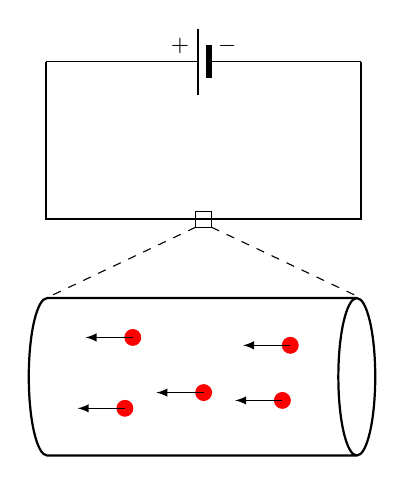
\begin{tikzpicture}
  % circuit
  \draw (-2,2) to[battery2] ++(4,0);
  \draw[thick] (2,2)
    to ++(0,-2)
    to ++(-4,0)
    to ++(0,2);
  \node at (-0.3,2.2) { \footnotesize $+$};
  \node at (+0.3,2.2) { \footnotesize $-$};
  % small window
  \draw (-0.1,-0.1) rectangle (0.1,0.1);
  % connection between small and large window
  \draw[dashed] (-0.1,-0.1) -- (-2,-1);
  \draw[dashed] (+0.1,-0.1) -- (+2,-1);
  \begin{scope}[yshift=-2cm]
    % cylinder
    \node[thick] (A) at (-0.2,0) [cylinder, aspect=2, shape border rotate=0, draw, minimum height=4.4cm, minimum width=2cm] {};
    % charges
    \foreach \x/\y in { -1/-0.4,-0.9/0.5,0/-0.2,1.1/0.4,1/-0.3 } {%
      \draw[fill,red] (\x,\y)  circle (0.1) coordinate (t);
      \draw[->] (t) -- ++(-0.6,0);
    }
  \end{scope}
\end{tikzpicture}
\end{document}
